% interacttfqsample.tex
% v1.05 - August 2017

\documentclass[]{interact}

\usepackage[table]{xcolor}
\usepackage{hyperref}
\usepackage{siunitx}
\usepackage{epstopdf}% To incorporate .eps illustrations using PDFLaTeX, etc.
\usepackage[caption=false]{subfig}% Support for small, `sub' figures and tables
%\usepackage[nolists,tablesfirst]{endfloat}% To `separate' figures and tables from text if required
%\usepackage[doublespacing]{setspace}% To produce a `double spaced' document if required
%\setlength\parindent{24pt}% To increase paragraph indentation when line spacing is doubled
%\setlength\bibindent{2em}% To increase hanging indent in bibliography when line spacing is doubled
\usepackage[numbers,sort&compress]{natbib}% Citation support using natbib.sty
\bibpunct[, ]{[}{]}{,}{n}{,}{,}% Citation support using natbib.sty
\renewcommand\bibfont{\fontsize{10}{12}\selectfont}% Bibliography support using natbib.sty

\theoremstyle{plain}% Theorem-like structures provided by amsthm.sty
\newtheorem{theorem}{Theorem}[section]
\newtheorem{lemma}[theorem]{Lemma}
\newtheorem{corollary}[theorem]{Corollary}
\newtheorem{proposition}[theorem]{Proposition}

\theoremstyle{definition}
\newtheorem{definition}[theorem]{Definition}
\newtheorem{example}[theorem]{Example}
\theoremstyle{remark}
\newtheorem{remark}{Remark}
\newtheorem{notation}{Notation}

\begin{document}

%\articletype{ARTICLE TEMPLATE}% Specify the article type or omit as appropriate

\title{MultIHeaTS : an Open Source Implicit Thermal Solver for 1D Heterogeneous Media}

\author{
\name{C. Mergny\textsuperscript{a}\thanks{CONTACT C. Mergny Email: cyril.mergny@universite-paris-saclay.fr} and F. Schmidt\textsuperscript{a,b}}
\affil{\textsuperscript{a}Université Paris-Saclay, CNRS, GEOPS, Orsay, France}
\affil{\textsuperscript{b}Institut Universitaire de France (IUF), Paris, France}
}





\maketitle

\begin{abstract}
An implicit scheme is proposed for solving heat conduction problems in 1D  heterogeneous media.
The algorithm uses finite difference on an irregular grid and is unconditionally stable due to the implicit formulation.
Boundary conditions can be either imposed temperature or flux. 
The algorithm was validated against an analytical solution and by comparison with existing algorithms \cite{Spencer1989, Schorghofer2010}.
For black body equilibrium, an explicit formulation of the upper boundary condition was used, which introduced some errors but keeps the scheme stability (cite).
Although the Crank-Nicolson \cite{Crank} scheme is generally considered more reliable for homogeneous media (citer), our numerical study shows that the proposed implicit scheme can be more accurate for large timesteps with fixed thermal properties and grid, and is also more reliable for handling stiff conditions.
\end{abstract}

\begin{keywords}
Sections; lists; figures; tables; mathematics; fonts; references; appendices
\end{keywords}


\section{Introduction}

The heat equation is a fundamental partial differential equation that governs the behavior of heat transfer in various physical systems. In the context of heterogeneous media, where the thermal properties of the material vary spatially, the heat equation becomes a challenging problem to solve.  In one dimension, the general form of the heat equation is expressed as :
\begin{equation}
    \rho(x, t) c_p(x, t) \dfrac{\partial T(x, t)}{\partial t} =  \dfrac{\partial}{\partial x} \left( k(x, t) \dfrac{\partial}{\partial x} T(x, t) \right)
    +  Q(x, t)
\end{equation}
%(preciser que c'est pas non lineaire). 
where $T$ is the temperature, $\rho$ is the density, $c_p$ the heat capacity, $k$ the thermal conductivity and $Q$ an optional source or sink term.
We want to solve this equation when all the thermal properties can vary (continously) over space and time and with non constant time and space increments. 

Several numerical methods exist to solve the heat equation for heterogeneous media, and have been explore in multiple research papers including finite element methods \cite{citer} and finite difference schemes \cite{citer}.
In this paper we focus on finite difference schemes which can be divided into three categories Explicit (Forward Euler), Implicit (Backward Euler) and Crank-Nicolson \cite{Crank1947}.
 The explicit method is easier to implement numericaly, has a faster computational time but its main disadvantage is its conditional stability. For 1D heterogeneous media, an implementation of the Explicit Scheme by Spencer \cite{Spencer1989}. 
The Crank-Nicolson is more complex to implement and as for the implicit scheme it requires a matrix inversion which makes it slower. On the other hand it is unconditionally stable and more precise than the other two schemes for homogeneous media. 
For 1D heterogeneous media  the Crank-Nicolson scheme was implemented in \cite{Schorghofer2010}.
Although the implicit scheme is also unconditionally stable, to our knowledge there does not exist any code available online which uses it to solve the heat equation in a heterogeneous media.
Therefore, our goal is to provide the scientific community with an open-source, easy-to-use and versatile implicit solver called MultIHeaTS (Multi-layered Implicit Heat Transfer Solver) for solving the heat equation in such conditions.
Although the target science is planetary science with surface condition subject to solar illumination, this approach is applicable in a wide range of scientific and technical cases.

In the first part of this paper we start by describing the mathematical derivation of the heat equation using our implicit schemes, then the algorithm is validated both using analytical solution and existing algorithm. We then discuss the accuracy and why our implicit scheme is more accurate than CN.

\section{Methods}


To discretize the heat equation we used finite differences on a irregular space grid made of $n_x$ points that we will iterate for a number of $n_t$ iterations. 
The space and time parameters are discretized as such :
\begin{equation}
\begin{cases}
    x \rightarrow x_n &= x_{n-1} + \Delta x_n \\
    t \rightarrow t^i &= t^{i-1} + \Delta t^i \\
    
\end{cases}
\end{equation}
with $n$ an integer such that $n \in  \{1, \: \dotsc \: , n_x\} $ representing the $n$th element in the spatial dimension, and $i$ an integer such that $i \in  \{1, \: \dotsc \: , n_t\} $, representing the $i$th element in the time dimension.
Note that both the spatial $\Delta x_n$ and time $\Delta t^i$ increments  may be taken non constant.

\subsection{Finite Differences on an Irregular Grid}

Following the method described in \cite{Sundqvist1970}, the first order derivative of function $f$ using the central difference approximation can be written as :
\begin{equation}
\frac{\partial f}{\partial x} (x_n) = \frac{f_{n+1}- f_{n}}{2 \Delta x_n} + \frac{f_{n}- f_{n-1}}{2 \Delta x_{n-1}} + \mathcal{O}(\Delta x_n^2)
 \label{eq:1_deriv}
\end{equation}
and the second order derivative as :
\begin{equation}
	\frac{\partial f^2}{\partial x^2} = \dfrac{2 \left( f_{n+1} \Delta x_{n-1} + f_{n-1} \Delta x_{n} - f_n \left( \Delta x_{n} + \Delta x_{n-1}\right) \right) }{\Delta x_{n} \Delta x_{n-1} \left( \Delta x_{n} + \Delta x_{n-1}\right)} + \mathcal{O}(\Delta x_n^3)
 \label{eq:2_deriv}
\end{equation}


Using equations \ref{eq:1_deriv} and \ref{eq:2_deriv}, the discretized version of the heat equation, after factorising each temperature terms can be written as :
\begin{align}
\begin{split}
	T_n^i + r_n^i Q_n^i = &T_{n-1}^{i+1}  \left[ \frac{-r_n}{\Delta x_{n-1}} \left( - \frac{1}{2} \frac{\partial k}{ \partial x} + \frac{2 k_n}{\Delta x_n + \Delta x_{n-1}} \right)  \right] \\
	+ &T_{n}^{i+1} \left[ 1 - \frac{r_n}{\Delta x_{n}\Delta x_{n-1}} \left( \frac{\left(\Delta x_{n}- \Delta x_{n-1} \right)}{2} \frac{\partial k}{ \partial x} - 2 k_n \right) \right] \\
      + &T_{n+1}^{i+1}\left[ \frac{-r_n}{\Delta x_{n}} \left( \frac{1}{2} \frac{\partial k}{ \partial x} + \frac{2 k_n}{\Delta x_n + \Delta x_{n-1}} \right) \right]
\end{split}
    \label{eq:dis_heat}
\end{align}
with $r_n$ a coefficient expressed as $r_n^i = \Delta t^i / (\rho_n^i c_n^i)$.
\textcolor{red}{Change notation $r_n$ and r seems like the same thing but not exactly!}
With matrix notation this is equivalent to the system :
\begin{equation}
    \begin{pmatrix}
    b_1 & c_1 & &  &\hdots  & & 0  \\
    a_2 & b_2 & c_2 &  \\
      &\ddots & \ddots & \ddots     \\
    \vdots  &  & a_n & b_n & c_n & &  \vdots \\
    & & &\ddots & \ddots & \ddots     \\
    & & &  & a_{n_x-1} & b_{n_x-1} & c_{n_x-1} \\
    0 & &  \hdots & & & a_{n_x} & b_{n_x}  \\
    \end{pmatrix}
    \cdot
    \begin{pmatrix}
    T_{1} \\
    \vdots \\
    T_{n-1} \\
    T_{n}  \\
    T_{n+1} \\
    \vdots \\
    T_{n_x}
    \end{pmatrix}^{i+1}
     = 
     \begin{pmatrix}
        s_{1} \\
        \vdots \\
        s_{n-1} \\
        s_{n}  \\
        s_{n+1} \\
        \vdots \\
        s_{n_x}
        \end{pmatrix}^{i}
\end{equation}
where the coefficients $a_n$, $b_n$, $c_n$ and $s_n$ are given by
\begin{equation}
\forall n \in [2, N-1] 
\begin{cases}
& a_n =   \dfrac{-r_n}{\Delta x_{n-1}} \left( - \dfrac{1}{2} \dfrac{\partial k}{ \partial x} + \dfrac{2 k_n}{\Delta x_n + \Delta x_{n-1}} \right) \\
& b_n = 1 - \dfrac{r_n}{\Delta x_{n}\Delta x_{n-1}} \left( \dfrac{\left(\Delta x_{n}- \Delta x_{n-1} \right)}{2} \dfrac{\partial k}{ \partial x} - 2 k_n \right) \\
& c_n =  \dfrac{-r_n}{\Delta x_{n}} \left( \frac{1}{2} \dfrac{\partial k}{ \partial x} + \dfrac{2 k_n}{\Delta x_n + \Delta x_{n-1}} \right)\\
& s_n = T_n^i + r_n^i Q_n^i\\
\end{cases}
\end{equation}
and by the boundary conditions.


\subsection{Boundary Conditions}

MultIHeaTS can accept any type of boundary conditions either imposed flux or imposed temperatures at the boundaries.
For a detailed derivation of the Dirichlet boundary conditions see Suplementary Materials \ref{sup:flux}.
As we are particularly interested in planetary surface evolution we will derive here the Neumann boundary conditions (imposed flux).
The flux is given at the boundaries meaning that
\begin{equation}
    \forall t, k_1 \left. \dfrac{\partial T(x, t)}{\partial x}\right|_{x_1} = \phi_1(t).
    \label{eq:upper_flux}
\end{equation}
By injecting equation \ref{eq:upper_flux} into the discretized heat equation \ref{eq:dis_heat}, the upper boundary condition becomes:
\begin{equation}
    T_1^{i+1} = T_1^i + r_1^i \left[ \Delta x_{1} \phi_1^{i+1} \left(k_{2}^i - 3k_{1}^i\right) + \Delta x^2_1 Q_n^i \right]
      +  2 r_1^i k_1^i T_{2}^{i+1} - 2 r_1^i k_1^i  T_{1}^{i+1}
\end{equation}
which gives the expression of the first coefficients of the tri-diagonal matrix :
\begin{equation}
    \begin{cases}
        &b_1 = 1 + 2 r_1 k_1 / \Delta x_1^2  \\
        &c_1 = - 2 r_1 k_1   / \Delta x_1^2 \\
        &s_1 =  T_1^i + r_1 \left( \phi_1 \left(k_{2} - 3k_{1} \right)/\Delta x_1 +  Q_n \right) \\
    \end{cases}   
\end{equation}
The same reasoning can be applied for the bottom boundary condition :
\begin{equation}
    \forall t, \left. \dfrac{\partial T(x, t)}{\partial x}\right|_{x_{n_x}} = \phi_b(t) 
\end{equation}
%\begin{equation}
%T_N^{i+1} = T_N^i + r_N^i \left[  \Delta x \phi_N^{i+1} \left(3k_{N}^i - k_{N-1}^i\right)  +  \Delta x^2 Q_n^i\right]
%+  2k_N^i r_N^i T_{N-1}^{i} - 2k_N^i r_N^i T_{N}^{i}
%\end{equation}
which gives the expression of the last tri-diagonal coefficients :
\begin{equation}
    \begin{cases}
        &a_{n_x}^i = - 2k_{n_x}^i r_{n_x}^i  \\
        &b_{n_x}^i = 1 +  2k_{n_x}^i r_{n_x}^i  \\
        &s_{n_x}^i =T_{n_x}^i + r_{n_x}^i \left[  \Delta x_{n_x} \phi_{n_x}^{i+1} \left( 3 k_{n_x}^i - k_{n_x-1}^i\right)  +  \Delta x^2_{n_x} Q_{n_x}^i\right] \\
        
    \end{cases}   
\end{equation}

\textcolor{red}{In cases where the flux is temperature dependant (like when there's black body radiation), the expression should not work (see Spencer). However, if we pre-calculate the surface flux using the previous temperature, the implicit can remain stable (in certain conditions) although this condition was expressed explicitly.}

\textcolor{red}{Talk about Cranck Nicolson here?}

\subsection{Stability and Errors}

\section{Results}

\subsection{Validation with an Analytical Solution}

Validation of our model using known analytical solutions of the heat equation can be achieved for homogeneous profiles only.
%In the case of constant conductivity, density and heat capacity the 1D heat equation can be solved analytically for a given set of initial and boundary conditions.
if we consider a stiff initial condition given by a step function defined on $[0, L]$ by the expression :
\begin{equation}
    \forall x \in [0, L], \, T(x, 0) = \left\{
\begin{array}{ll}
0, & \text{if } x < L/2 \\
1, &  \text{if } x \geq L/2.\\
\end{array}
    \right.
\label{eq:step_fct}
\end{equation}
then the analytical solution with zero-flux boundary conditions can be obtained (detailed derivation in Supplementary Materials \ref{sup:ana}) through Fourier series decomposition :
\begin{equation}
    T(x, t) = \frac{1}{2} - \sum_{j=1}^{+\infty} \frac{2}{\pi j} \sin\left(\frac{\pi j}{2}\right) \cos\left(\frac{\pi j x}{L}\right)    e^{-\alpha \left(\dfrac{ \pi j}{L} \right)^2 t}
\end{equation}
where $\alpha$ is the thermal diffusivity expressed as $\alpha= k / \rho c_p$.

\begin{figure}[htpb]
	\centering
	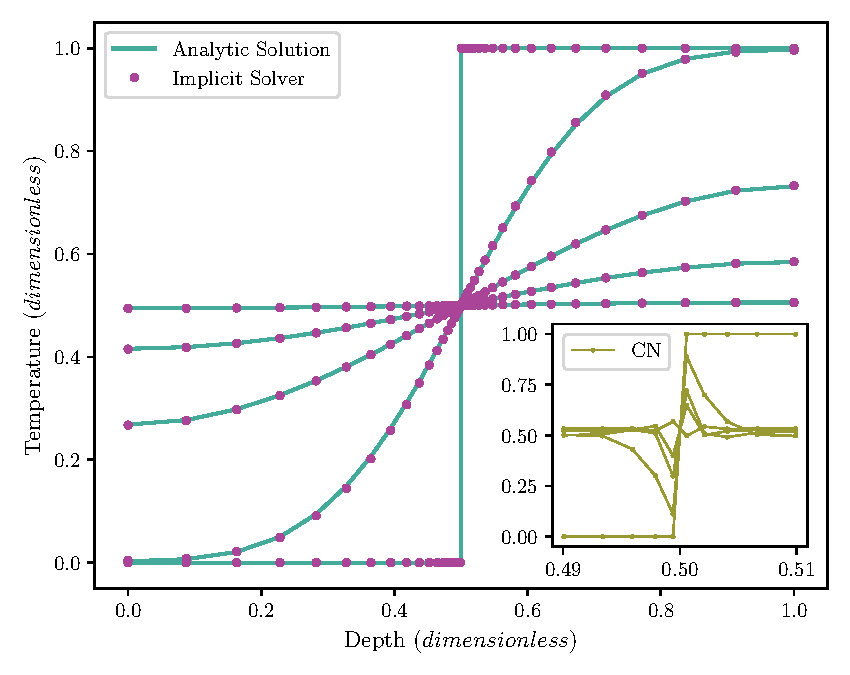
\includegraphics[width=0.8\textwidth]{figures/valid_ana.pdf}
	\caption{Analytical validation for a stiff initial condition and homogeneous thermal properties on an irregular grid. Despite the discontinuity at $x = 0.5 $, the implicit solver MultIHeaTS can compute the evolution of temperature with a very close match  ($e_+< 0.5\%$) to the analytic solution. (\textit{Bottom Right}) Zoom on the spurious oscillations of the Crank-Nicolson solver at the location of the initial discontinuity. }
	\label{fig:valid_ana}
\end{figure}

To validate our model, we need to compare the computed temperatures with the analytical solutions for the same set of thermal parameters. This is done by computing the error, defined as the absolute value of difference between the temperature produced by the numerical model $T$ and the reference temperature $\theta$. The maximum error $e_+$ is expressed as : 
\begin{align}
    e_+ = \max_{i,n} \left| T^i_n - \theta^i_n \right|
\end{align}
and the average error $\overline{e}$ as :
\begin{equation}
    \overline{e} = \frac{1}{n_x n_t} \sum_{n, i}^{n_x,n_t}\left| T^i_n - \theta^i_n \right|
\end{equation}
with $\theta^i_n$ the reference temperature taken at the exact same location $x_n$ and time $t^i$.
For proper validation, both the numerical solver and the reference solution need to be calculated until the reach of a stationary regime, with exactly the same thermal properties and conditions (see figure \ref{fig:valid_ana}). \
For a set of $n_x= 40$ grid points of constant diffusivity $\alpha \approx \SI{0.55}{m^2.s^{-1}}$ and $n_t=700$ iterations of timestep $\Delta t = 1000 \:  r_c$, the maximum error $e_+$ between the analytical solution and the implicit solver is less than 0.5\% and the mean error $\overline{e}$ is under 0.02\%.  
Results show a very close fit between the numerical and analytic solutions which proves that the MultIHeaTS model works well for homogeneous media.

The same test was realised using  Crank-Nicolson solver \cite{Schorghofer2010} to test its robustness to stiff initial conditions. 
Using the same parameters as previously, the Crank-Nicolson solver appears to create spurious oscillations located where the initial discontinuity was found (Figure \ref{fig:valid_ana}, \textit{Bottom Right}). 
The maximum error $e_+$ between the analytical solution and the Crank-Nicolson solver goes up to 38\% and the mean error $\overline{e}$ averages 3\%. 
These oscillations disappear slowly after some time \cite{citer}.   These results shows that although the Crank-Nicolson solver is more accurate that the implicit one for homogeneous media (error in ) \cite{citer}, for situations with stiff equations \cite{citer} it is more reliable to use an implicit solver.
\textcolor{red}{Further studies (or previous) could look at which temperature gradient the Crank-Nicolson starts oscillating.}


\subsection{Validation by Comparison with Explicit Scheme}

In more complex cases, in particular when the conductivity is depth dependant, analytic solutions of the heat equation do not exist. 
In these cases, validation of the model comes from comparaison with experimental data and/or  other previously well established numerical algorithms.
As our target application is to study realistic planetary surfaces conditions, we chose to compare our method with Spencer's \cite{Spencer1989} explicit scheme, an algorithm commonly used by planetary scientists.
Spencer's algorithm was written in IDL and is accessible on his personal website \footnote{\url{https://www.boulder.swri.edu/~spencer/thermprojrs/}}.

To compare these two models well, we need to make sure that the thermal properties are identical and that the boundary conditions are the same.
Notably for planetary surfaces, the solar flux  $F_{solar}$ is responsible for the temperature evolution.
Spencer chose to approximate the heating of a planet surface by the Sun throughout a sidereal day by a truncated sinusoidal function :
\begin{equation}
	F_{solar}(t) = \left\{ 
		\begin{array}{ll}
			\left(1 - A \right) \dfrac{G_{sc}}{d^2} \cos \left(\dfrac{2 \pi t}{P} \right) & \text{ if } {2 \pi t}/{P} \text{ in } \left[-\frac{\pi}{2}, \frac{\pi}{2}\right] \\ 
		\text{or} \\
		0   &  \text{ if }  {2 \pi t}/{P} \text{ in } \left]\frac{\pi}{2}, \frac{3\pi}{2}\right[ \\
		\end{array}
	\right.
\end{equation}
where $A$ is the albedo, $G_{sc}$ the solar constant and $d$ the distance between the Sun and the planet. 
The upper boundary condition (the flux leaving the surface) is then given by the energy equilibrium between the solar flux and the suface black body emission :
\begin{equation}
    \forall t, k_1 \left. \dfrac{\partial T(x, t)}{\partial x}\right|_{x_1} =  - F_{solar}(t) + \epsilon \cdot \sigma_{SB} \cdot T(0, t)^4
\end{equation}
where $\epsilon$ is the emissivity and $\sigma_{SB}$ the Stefan-Boltzmann constant.

\begin{table}[htbp]
    \centering
    \begin{tabular}{ l l c c l } 
     \hline
     Thermal Properties & Unit & Top value & Bottom value & Interface \\ 
     \hline
     Density $\rho$ & kg.m$^{-3}$ & 800 & 2000 & 25 cm \\ 
    Heat Capacity $c_p$ & J.kg$^{-1}$.K$^{-1}$ & 600 & 1800 & 50 cm \\ 
    Inertia $I_{th}$ & J.m$^{-2}$.K$^{-1}$.s$^{-1/2}$ & 200 & 20 & 100 cm \\ 
     \hline
    \end{tabular}
\caption{Thermal properties used for comparison of Spencer's explicit algorithm with MultIHeaTS. Although some of these values are close to what could be found on realistic icy surfaces, they were varied over large scales for validation purposes.}
\label{tab:thermal_ppties}
\end{table}

\begin{figure}[htpb]
	\centering
	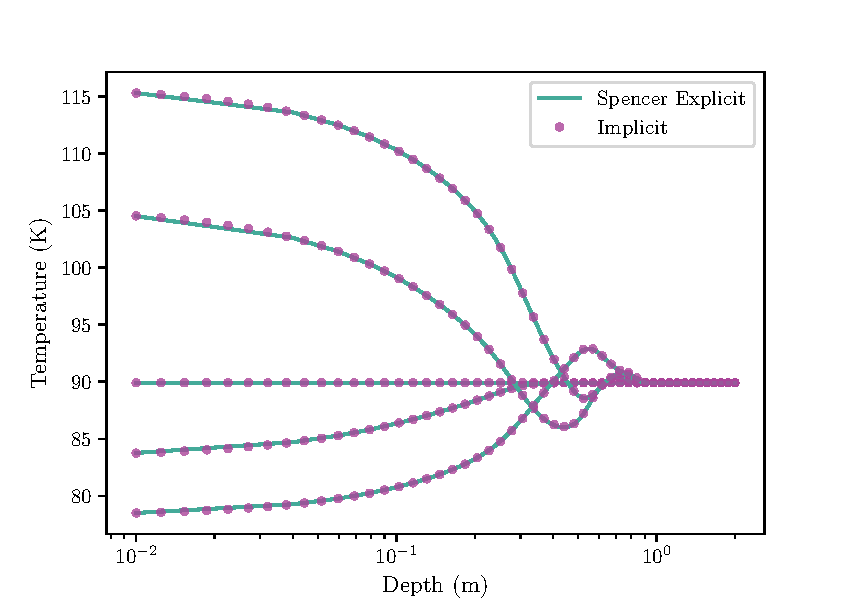
\includegraphics[width=0.8\textwidth]{figures/valid_spencer.pdf}
	\caption{Validation of MultIHeaTS with Spencer's explicit algorithm. Temperature profiles for different times are plotted simultaneously. MultIHeaTS is as accurate as Spencer's explicit scheme with the advantage of being unconditionally stable. 
    Note the uneven grid spacing of the implicit scheme, denser at the surface, shown by the logarithmic horizontal axis.
    }
    \label{fig:val_spencer}
\end{figure}

For the sake of validation, values of density, heat capacity and conductivity are varied through the depth by the largest scales allowed by Spencer's explicit scheme stability criteria (see Table \ref{tab:thermal_ppties}).
Both algorithm were run with meticulous attention with the exact same parameters that can be found in Table \ref{tab:params}. Notably the simulations are run on a $\SI{2}{m}$ thick grid consisting of $n_x=100$ points for $n_t = 5 \times 10^4 $ iterations, with a computational time less than 1 min on a intel CPU i7-10750.

Overall, results (see Figure \ref{fig:val_spencer}) show  a very good adequation between the explicit and implicit schemes, with little to no variations between both temperature profiles. 
The maximum error  between MultIHeaTS and the Spencer's solver is $e_+=0.68\%$ and the mean error is $\overline{e}=0.052\%$.
\textcolor{red}{Errors are mostly concentred near the surface (in opposition to CN where they are at the highest temperature gradient, near the bi-layer interface.}
These results show that our implicit model can compute accurately the same temperature profiles as Spencer's explicit algorithm, without the limitations of conditional stability.




\subsection{Comparison with Crank-Nicholson for Heterogeneous Media}

A numerical implementation of the Crank-Nicolson scheme for heterogeneous planetary surfaces has been developed by Schorghofer \cite{Schorghofer2010} and is accessible online on his Github repository\footnote{\url{https://github.com/nschorgh/Planetary-Code-Collection}}. 
The Crank-Nicolson scheme also has the advantage of being unconditionally stable, and for homogeneous media it is more accurate \cite{citer} and computationally more efficient than the implicit scheme \cite{citer}.  \textcolor{red}{Ref to the truncation error paragraph.}
However for more complex and realistic cases, like heterogeneous surfaces subject to surface energy equilibrium  it is unclear whether Crank-Nicolson remains the most reliable. \textcolor{red}{Notably due to the non linearity induced by black body emission.}

\begin{figure}[htpb]
	\centering
	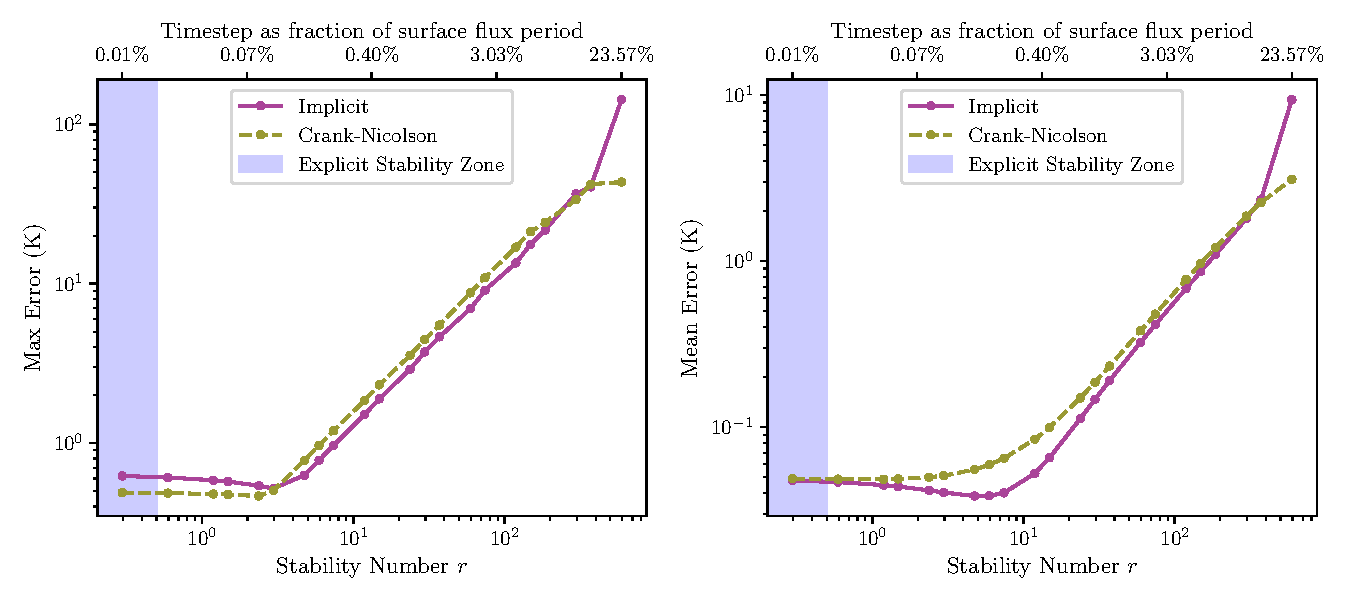
\includegraphics[width=1.0\textwidth]{figures/solver_compare.pdf}
	\caption{Errors produced by the Crank-Nicholson and our MultIHeaTS implicit scheme in comparison to Spencer's implicit model as functions of the timesteps $\Delta t$ used. Average temperature is around $\SI{90}{K}$. Timestep is represented as a fraction of the surface flux' period at the top and by the dimensionless number $r=\alpha \Delta t / \Delta x^2$ at the bottom. The stability zone of the explicit scheme $r< 1/2$ is represented in light blue. (Left) Maximum error $e$ produced by both solvers. (Right) Mean error $<e>$ produced by both solvers. Note that axis are in log/log.
 }
	\label{fig:solvers_comp}
\end{figure}

In this paragraph, we propose a numerical study to compare the behaviors of both our MultIHeaTS solver and Schorghofer Crank-Nicolson scheme outside the stability zone of the explicit algorithms (see Figure \ref{fig:solvers_comp}).
Our goal is to look at the evolution of errors produced by both algorithms with respect to the increase of the time step. 
To do so we ran, as a reference, Spencer's explicit algorithm for a small timestep $\Delta t = P / (5 \times 10^4)$. Each time the timestep is increased, the algorithms looses information which induces differences in regards to the accurately computed temperatures from Spencer.
\textcolor{red}{Du mal a bien formuler de maniere concise cet experience...}
Apart from the variable timestep $\Delta t$ and number of iterations $n_t$, the properties and parameters used here are the same as for the previous experiments and can be found respectively on Table \ref{tab:thermal_ppties} and \ref{tab:params}.

First we can notice that thanks to the unconditional stability of both algorithm we can extend the domain of computation to 100 times the stability zone while keeping a reasonable error. \textcolor{red}{Improve sentence? Give arbitrary error threshold ?}
In every cases, the Crank Nicolson is on average 30\% computationally faster than our implicit algorithm.
For small timesteps near the explicit stability zone, Schorgofer's Crank-Nicolson ($e_+=0.53\%$, $\overline{e} = 0.054\%$) and our MultiHeaTS algorithm ($e_+=0.68\%$, $\overline{e} = 0.052\%$) are almost equivalent with a slightly lower maximum error for Crank-Nicolson. 
For larger timesteps, at fixed grid and thermal properties, the difference of errors becomes more noticeable. 
Around $r=1$ to $r=100$, MultiHeaTS is more accurate both on average and for the maximum error.
Above the $r=100$ threshold, the errors produced by both algorithms become too high for the output temperatures to be relevant.
\textcolor{red}{Discuss why error decreases at first for implicit ?}


These findings suggest that when dealing with time steps that exceed the explicit stability zone, our implicit solver MultiHeaTS seems to be more accurate than the Crank-Nicolson solver.
This is particularly interesting for planetary studies,  where it is often necessary to examine temperature evolution over several years ($t^{n_t} \gg P$). 
 In such cases, it is computationally too expensive to attain a precise timestep for the diurnal evolution highlighting the need for a more accurate solver when dealing with larger timesteps.

 



\section{Conclusion}
We have implemented an open-source implicit algorithm called MultIHeaTS, that uses finite differences to solve the heat equation on 1D heterogeneous media with an irregular grid.
Although our target goal is planetary science, our algorithm is flexible and accommodates for different types of boundary conditions and thermal profiles. 

For homogeneous cases, the algorithm was validated using a known analytical solution.
This validation which used a discontinuous initial equation showed the robustness MultIHeaTS to stiff equations, in contrary to the Crank-Nicolson scheme.
For heterogeneous cases, MultIHeaTS was validated by comparison to a well established explicit algorithm in planetary science \cite{Spencer1989}.
Although our explicit formulation of the surface energy equilibrium condition, our implicit scheme remained accurate and stable, showing a very close match to Spencer's model.

Thanks to its unconditional stability, this implicit scheme allow us to extend the stability domain by 2 orders of magnitude, above which the truncation error becomes significant.
In a numerical the study, we compared the errors produced by our algorithm with an existing implementation of the Crank-Nicolson scheme by Schorghofer \cite{Schorghofer2010}.
Our results show that when the timestep increases, at fixed grid size and thermal properties, our MultIHeaTS solver becomes more accurate than Crank-Nicolson.

The MultIHeaTS algorithm has a wide range of potential applications, and its open-source and flexible nature make it adaptable to various domains. In planetary science, it is expected to be useful for retrieving thermal properties of multi-layered planetary surfaces using brightness temperature data but it can also be coupled with other physical processes to study the evolution of icy surfaces. 

\section*{Acknowledgement}
We acknowledge support from the ``Institut National des Sciences de l'Univers'' (INSU), the ``Centre National de la Recherche Scientifique'' (CNRS) and ``Centre National d'Etudes Spatiales'' (CNES) through the ``Programme National de Plan{\'e}tologie''. 


\newpage
\section*{Figures}

\begin{itemize}
    \item parler de la truncation error en O(dt2) pour equation classique (ie homogene) !!
    \item introduire nombre de stabilité.Parler dans un autre paragraph du critère de stabilité de l'explicite.
    \item parler du growth factor et le citer ?
    \item voir aussi  \url{http://hplgit.github.io/num-methods-for-PDEs/doc/pub/diffu/html/._diffu001.html}
    \item parler de condition limite explicite et de sa stabilité.
    \item parler de la ou se trouve l'erreur principalement sur Crank Nicolson ?
    \item Citer (Crank and Nicolson, 1947; Press et al., 1992)
    \item  \textcolor{red}{Talk about CN boundary condition: predictor-corrector.}
\end{itemize}


\bibliography{library}
\bibliographystyle{tfq.bst}


\section*{Appendices}

\subsection{Dirichlet boundary conditions:}
The temperature is fixed at the boundaries which gives us at the top boundary $x=a$:
\begin{equation}
    \forall t, T(a, t) = T_a(t) \implies
    \begin{cases}
        &b_1^i = 1 \\
        &c_1^i = 0 \\
        &s_1^i = T_a^i, \\
    \end{cases}  
\end{equation}
at at the bottom boundary $x=b$,
\begin{equation}
    \forall t, T(b, t) = T_b(t) \implies
    \begin{cases}
        &a_N^i = 0 \\
        &b_N^i = 1 \\
        &s_N^i = T_b^i. \\
    \end{cases}  
\end{equation}


\subsection{Analytic Solution}
\label{sup:ana}
\subsubsection{Fourier series}
Any periodical function $f$ in $\mathbb{R}$ of period $P$ can be written as a Fourier series:
\begin{equation}
    f(x) =  \frac{a_0}{2} + \sum_{n=1}^{+\infty} a_n \cos\left(\frac{2\pi n x}{P}\right) + b_n \sin\left(\frac{2\pi n x}{P}\right),
    \label{eq:fourier_series}
\end{equation}
with the coefficients $a_n$ and $b_n$ given by the expressions:
\begin{equation}
    a_n = \frac{2}{P} \int_P f(x) \cos\left(\frac{2\pi n x}{P}\right) dx,
    \label{eq:a_n}
\end{equation}
\begin{equation}
    b_n = \frac{2}{P} \int_P f(x) \sin\left(\frac{2\pi n x}{P}\right) dx.
    \label{eq:b_n}
\end{equation}
The expressions are obtained by integrating equation (\ref{eq:fourier_series}) as demonstrated here:
\begin{align*}
    \int_P f(x) \cos\left(\frac{2\pi m x}{P}\right) dx & =  \int_P  \cos\left(\frac{2\pi m x}{P}\right)\left[ \frac{a_0}{2} + \sum_{n=1}^{+\infty} a_n \cos\left(\frac{2\pi n x}{P}\right) + b_n \sin\left(\frac{2\pi n x}{P}\right) \right] dx \\
    &=  \sum_{n=1}^{+\infty} \int_P  a_n \cos\left(\frac{2\pi n x}{P}\right)  \cos\left(\frac{2\pi m x}{P}\right) dx \\
    &= a_m \frac{P}{2}
\end{align*}

\subsubsection{Fourier series of a step function}
Every function on a interval of length $P$ can be extended to a periodic function in $\mathbb{R}$ of period $P$.
First we will extend function $H$ on the interval $[-\frac{L}{2}, \frac{3L}{2}]$ such that the derivative at $x=0$ and $x=L$ are equal to zero (Boundary flux condition). 
The step function is still defined by equation (\ref{eq:step_fct}) in $[-\frac{L}{2}, \frac{3L}{2}]$.

Then we use equations (\ref{eq:a_n}) and (\ref{eq:b_n}) with $P=2L$ the interval length to find the coefficient $a_n$ and $b_n$:
\begin{align*}
    a_n &= \frac{1}{L} \int_{-\frac{L}{2}}^{\frac{3L}{2}} H(x) \cos\left(\frac{\pi n x}{L}\right) dx \\
    & = \frac{1}{L} \int_{\frac{L}{2}}^{\frac{3L}{2}} \cos\left(\frac{\pi n x}{L}\right) dx \\
    & = \frac{-2}{\pi n} \sin\left( \frac{\pi n}{2} \right)
\end{align*}
and a similar integration for $b_n$ leads to $b_n=0$.
The step function can then be written as a Fourier series using equation (\ref{eq:fourier_series}):
\begin{equation}
    H(x) = \frac{1}{2} - \sum_{n=1}^{+\infty} \frac{4}{\pi n} \sin\left(\frac{\pi n }{2} \right) \cos\left(\frac{\pi n x}{L}\right).
\end{equation}

\subsubsection{Solving the heat equation by separation of variables}

The solution of the 1D heat equation (\ref{eq:1Dheateq}) with initial condition (\ref{eq:step_fct}), can be obtained by separation of variables. Let's assume that the solution can be written as
\begin{equation}
    T(x, t) = v(x)w(t)
\end{equation}
with $v$ and $w$ functions of $x$ and respectively $t$. This expression injected int the heat equation results to:
\begin{equation}
   v(x) \dfrac{\partial w(t)}{\partial t} = \alpha  \dfrac{\partial^2 v(x)}{\partial x^2} w(t)
\end{equation}
This first order differential equation as for $w$ the general solution:
\begin{equation}
    w(t) = w(0) e^{\alpha \dfrac{v^{''}(x)}{v(x)} t}
\end{equation}
where $v^{''}$ is the second derivative of $v$ with respect to $x$. If we take $v(x) = T_n(x, 0) = f_n(x)$ the initial function decomposed in 
a Fourier series, then we have:
\begin{equation}
        v^{''}(x) = -\left(\frac{2 \pi n}{P} \right)^2 f_n(x)
\end{equation} 
and 
\begin{align*}
    & T(x, 0) = v(x)w(0) = f(x) \\
    & v(x) = f(x) \implies w(0) = 1
\end{align*}
which give us the exact express of the solution of $w$ with:
\begin{equation}
    w(t) = e^{-\alpha \left(\dfrac{2 \pi n}{P} \right)^2 t}
\end{equation}
Hence the solution is given by:

\begin{equation}
    T(x, t) = \frac{a_0}{2} + \sum_{n=1}^{+\infty} \left(a_n \cos\left(\frac{2\pi n x}{P}\right) + b_n \sin\left(\frac{2\pi n x}{P}\right) \right)  e^{-\alpha \left(\dfrac{2 \pi n}{P} \right)^2 t}
\end{equation}

\subsection{Parameters}
\begin{table}[htbp]
    \centering
    \begin{tabular}{ll}
    \hline
    Parameters & Value \\ 
    \hline
    Distance to Sun $d$ &  9.51 UA  \\
    Emissivity &  1  \\
    Albedo $A$ & 0.015  \\
    Grid points $n_x$ & 100  \\
    Max Depth  m & 2 m    \\
    Initial Temperature &  90 K  \\
    Solar Period $P$$  & 79.3 days   \\
    Number of Periods & 5   \\
    Number of iterations $n_t$ &   50000   \\
    \hline
    \end{tabular}
\caption{Physics and numerical parameters used for comparing Spencer algorithm with MultIHeaTS.}
\label{tab:params}
\end{table}




\end{document}
